\documentclass{article}
\usepackage{times}
\usepackage{graphicx} % more modern
\usepackage{subfigure}
\usepackage{natbib}
\usepackage{hyperref}
\usepackage[accepted]{grcon/grcon}

\usepackage{color}
\definecolor{grey}{rgb}{0.95,0.95,0.95}
\definecolor{keyword}{rgb}{0,0,0.55}
\definecolor{comment}{rgb}{0.55,0,0}
\definecolor{string}{rgb}{0,0.55,00.55}

\usepackage{listings}
\lstset{backgroundcolor=\color{grey},
        language=C,
        numbers=left,
        numbersep=6pt,
        basicstyle=\small\ttfamily,
        extendedchars=true,
        tabsize=3,
        keywordstyle=\color{keyword}\bfseries,
        commentstyle=\color{comment},
        stringstyle=\color{string}\itshape,
        columns=fullflexible, % fullflexible
        keepspaces=true
}

\grcontitlerunning{gr-rpitx: GNU Radio compatible general purpose SDR emitter using the Raspberry Pi}

\begin{document}

\twocolumn[
\grcontitle{gr-rpitx: GNU Radio compatible general purpose SDR emitter using the Raspberry Pi(4) internal phase locked loop}

\grconauthor{Jean-Michel Friedt}{jmfriedt@femto-st.fr}
\grconaddress{FEMTO-ST/Time \& Frequency, Besan\c con, France}
\grconauthor{\'Evariste Courjaud}{evaristec@gmail.com}
\grconaddress{}

\grconkeywords{Raspberry Pi, Buildroot, rpitx}
]

\vskip 0.3in

\begin{abstract}
{\tt gr-rpitx} provides the support for the full GNU Radio signal processing framework when
using the Raspberry Pi internal radiofrequency Phase Locked Loop (PLL) controlled by the Pulse
Width Modulation (PWM) Direct Memory Access (DMA) for tuning the output frequency. Furthermore,
the {\tt librpitx} added amplitude tuning. Thanks to frequency and amplitude tuning capability,
full IQ datastreams can be processed, here within the framework of a GNU Radio Sink block. We
promote {\tt gr-rpitx}, despite the multiple spurious spectral components preventing the emission
over the air, for educational purposes including emitting and recording analog and digital communication
mode or probing the transfer function of a device under test in a scalar vector network analyzer
configuration.
\end{abstract}

\section{Introduction}\label{submission}

Emitting radiofrequency signals from one of the Raspberry Pi (RPi) General Purpose Intput
Output (GPIO) pins has been known since 2012 with the release of {\tt PiFm} as described
at \url{http://www.icrobotics.co.uk/wiki/index.php/Turning_the_Raspberry_Pi_Into_an_FM_Transmitter}.
Incremental improvements have included adding amplitude $A$ tuning to frequency $f$ tuning, as
described at \cite{sdra}, leading to full IQ stream controlling the radiofrequency output
since $I=Re(I+jQ)=A\cos(\varphi)$ and $Q=Im(I+jQ)=A\sin(\varphi)$ with the phase
being the integral of the frequency $\varphi=\int f\cdot dt$. Packaging such functionalities
in a library with a blocking call to filling the DMA buffer makes the transition to GNU Radio
trivial, and yet opens the doors to streaming any signal generated by a GNU Radio Companion
flowchart. The educational benefits of this radiofrequency signal emission approach, when
coupled with the RTL-SDR Digital Video Broadcast-Terrestrial (DVB-T) dongles used as general
purpose Software Defined Radio (SDR) receivers, is significant as long as over-the-air emission
is avoided and only short range communication is allowed by the poor impedance matching of the
pin length with the radiofrequency wavelength of the emitted signal.

\section{Basics of the sink block}

The GNU Radio 3.8 Out Of Tree (OOT) module tree structure is generated with {\tt gr\_modtool}
with two arguments shared with the constructor, the sampling rate defining the rate which
DMA transfers will occur between the GNU Radio buffer and the hardware peripheral, and the
carrier frequency. The constructor allocates the DMA buffer, defines the nature of the exchanged
data and the carrier frequency. The main work function is reduced to a blocking call to filling
the buffer with the data transfered from the previous block. The scheduler is informed of the
timing capability of this sink block, thanks to the blocking call to the DMA filling function,
with the {\tt throttle} flag in the GNU Radio Companion YAML description of the block.

The Constructor initializes the DMA and datastream structure following the example
provided by {\tt sendiq} at \url{https://github.com/F5OEO/rpitx/blob/master/src/sendiq.cpp}

\begin{lstlisting}{language=C}
#define IQSize 4096

namespace gr {
 namespace rpitx {

 rpitx_source_impl::rpitx_source_impl(float 
  samp_rate, float carrier_freq): 
  gr::sync_block("rpitx_source",
  gr::io_signature::make(1,1,sizeof(gr_complex)),
  gr::io_signature::make(0, 0, 0))
   {iqtest=new iqdmasync(carrier_freq,samp_rate,
               14,IQSize*4,MODE_IQ);
    iqtest->SetPLLMasterLoop(3,4,0);
   }

rpitx_source_impl::~rpitx_source_impl()
  {iqtest->stop();
   delete(iqtest);
  }
\end{lstlisting}
which also includes the destructor definition to release resources. The {\tt work}
function is fed {\tt noutput\_items} to be transferred to the buffer as follows, using
the blocking {\tt iqtest$\rightarrow$SetIQSamples} to regulate the datarate when filling 
the DMA buffer:

\begin{lstlisting}{language=C}
int rpitx_source_impl::work(int noutput_items,
  gr_vector_const_void_star &input_items,
  gr_vector_void_star &output_items)
   {std::complex<float> CIQBuffer[IQSize];  
    int H=1; // Harmonic
    int nbread=0,xferlen;
    const gr_complex *in=\
          (const gr_complex*)input_items[0];

    while (nbread<noutput_items)
     {if (nbread+IQSize<noutput_items) 
         xferlen=IQSize; 
      else xferlen=noutput_items-nbread;
      iqtest->SetIQSamples((std::\
       complex<float>*)&in[nbread],xferlen,H);
      nbread+=xferlen;
     }
    return noutput_items;
   }
  } /* namespace rpitx */
} /* namespace gr */
\end{lstlisting}

This datarate regulation must be advertised to GNU Radio Companion to avoid
the missing Throttle block warning: the YAML description file includes
\begin{verbatim}
id: rpitx_rpitx_source
label: rpitx source
category: '[Rpitx]'
flags: throttle
...
\end{verbatim}
to let GNU Radio Companion know that this flow graph will regulate the
datastream \cite{flag}.

\section{Practical demonstration (1): analog FM broadcast}

FM broadcasting is demonstrated at
\url{https://www.youtube.com/watch?v=JIiKZ3UVAIw} in which the
signal emitted by {\tt gr-rpitx} (Fig. \ref{fm_grc}) is collected by a DVB-T dongle
connected to the RPi4 and streamed through a 0MQ socket to the
laptop PC used as a sound card to record the demodulated signal (Fig. \ref{fm}).

\begin{figure}[h!tb]
\includegraphics[width=\linewidth]{../examples/rpi_fm.pdf}
\caption{FM broadcast flowchart demonstrating the efficient integration of {\tt gr-rpitx}
with GNU Radio general purpose processing blocks.}
\label{fm_grc}
\end{figure}

In all these examples, ``No GUI'' flowcharts are assembled on the host PC generating 
the Python3 script which is transfered to the Raspberry Pi4 for execution on the target.

\begin{figure}[h!tb]
\includegraphics[width=\linewidth]{../examples/DSC_0600_4.JPG}
\caption{Experimental setup for assessing FM broadcasting from {\tt gr-rpitx}
and reception using a DVB-T receiver used as general purpose Software Defined Radio
receiver connected to the Raspberry Pi4 running GNU Radio. The demodulated output
audio stream is transferred to the host PC acting as a sound card for playing the
audio signal using a 0MQ publish-subscribe link.}
\label{fm}
\end{figure}

The maximum sampling rate we achieved on analog broadcast wideband FM 
transmission with no audible loss of quality or pitch is $48000\times 9=432$~kHz
while $48000\times 10=480$~kHz led to an obvious slow-down of the output stream.
On the other hand, a continuous wave (CW) signal source streaming a 70~kHz sine
wave at a rate of 3.42~MS/s at 87 MHz brought to baseband by Xlating FIR
demonstrated a continuous transmission and no spreading by discontinuous
acquisition, while no at all was transmitted at 3.43 MS/s. 

\section{Practical demonstration (2): digital (DRM) broadcast}

\begin{figure*}
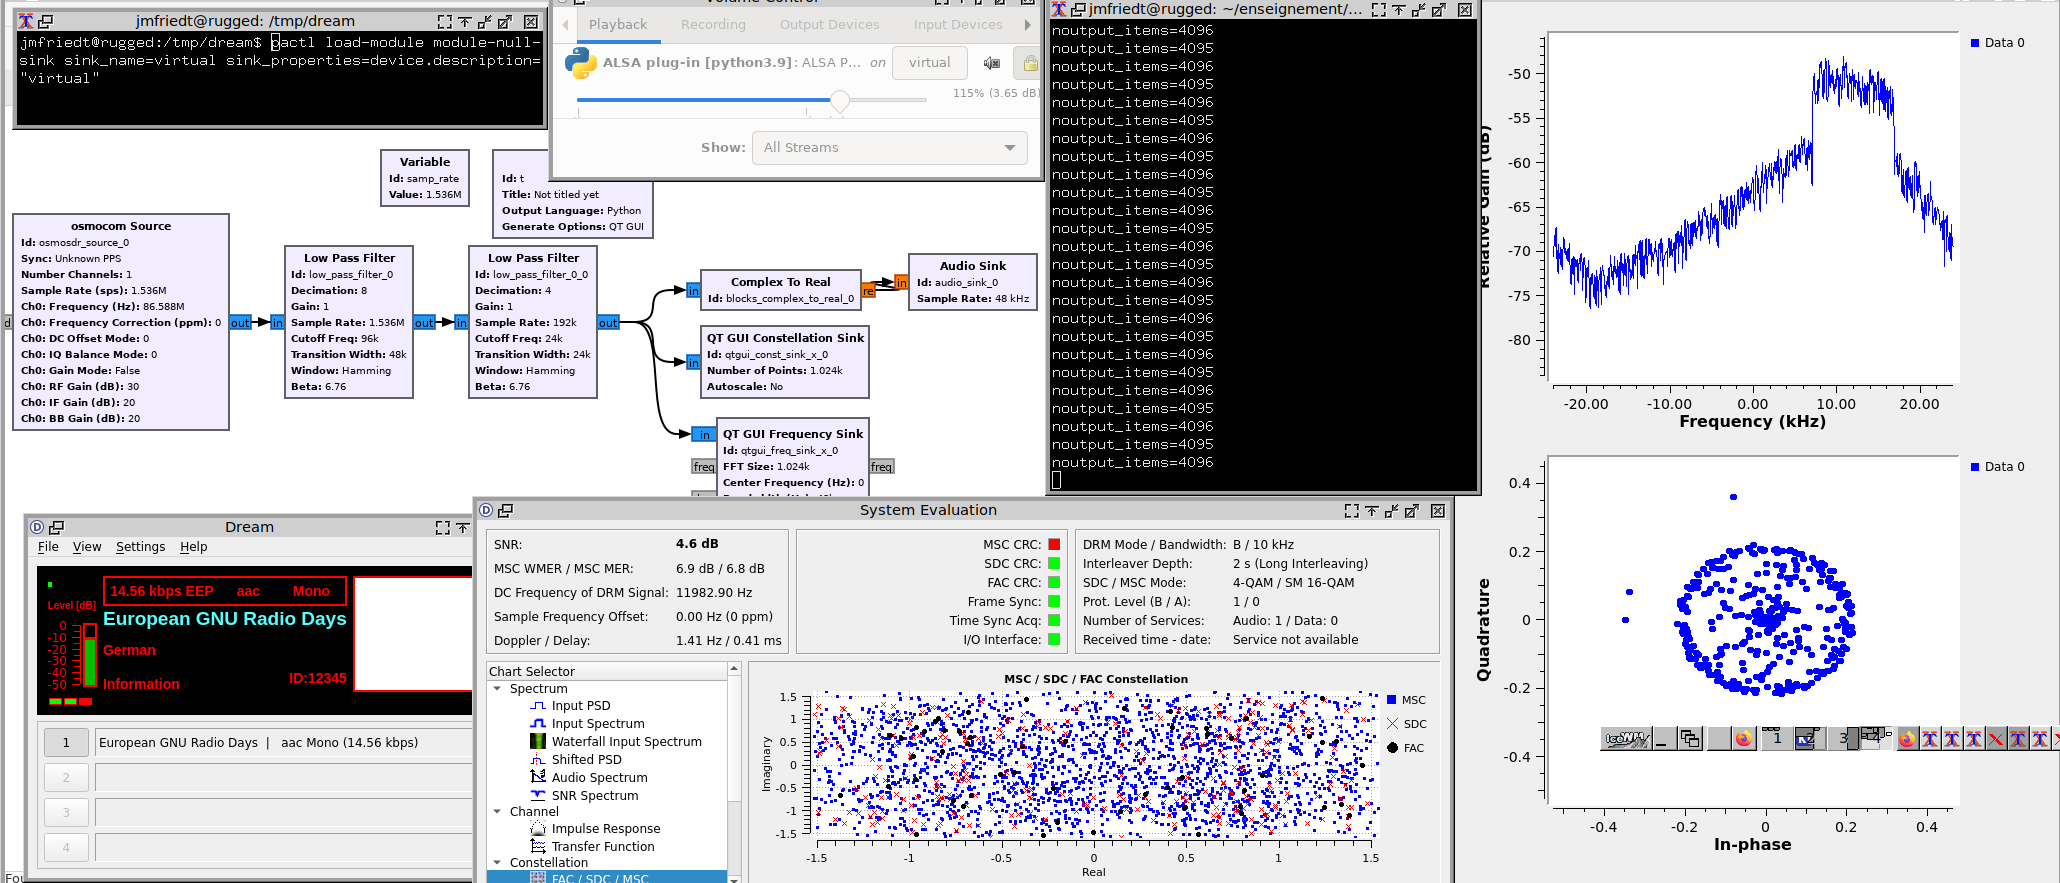
\includegraphics[width=\linewidth]{2021-05-05-072649_2624x900_scrot.png}
\caption{DRM (Digital Radio Mondiale) emission from {\tt gr-rpitx} fed
by {\tt gr-drm} and reception using DREAM running on the host PC. Notice how
a Pulse Audio virtual sink is used to feed DREAM with the output of GNU Radio.
Right is the spectrum (magnitude) and raw constellation observed with GNU Radio,
center-bottom is the constellation provided by DREAM, bottom left demonstrates
how the encoding and station identified are decoded, top left is the host PC
reception scheme and top left is the Pulse Audio virtual sink while top-middle is
the Raspberry Pi 4 terminal emitting DRM using {\tt gr-rpitx}. The signal to noise
ratio is below 5~dB, preventing the constellation from locking on the audio signal.}
\label{drm}
\end{figure*}

As radiofrequency communication is shifting from analog to the more
efficient spectrum occupation digital modulation schemes, we extend
the analog FM broadcast demonstration to a digital mode. While Digital
Audio Broadcast (DAB) requires excessive bandwidth to be compatible
with {\tt gr-rpitx}, Digital Radio Mondiale (DRM \cite{drm}) provides an acceptable
tradeoff between simplicity, availability and bandwidth. Running {\tt gr-drm}
as found at \url{https://github.com/kit-cel/gr-drm} is as simple as replacing
the UHD sink of the sample example -- already clocking the datastream at
an acceptable 250~kHz -- to the {\tt gr-rpitx} sink (Fig. \ref{drmtx}). 

\begin{figure}[h!tb]
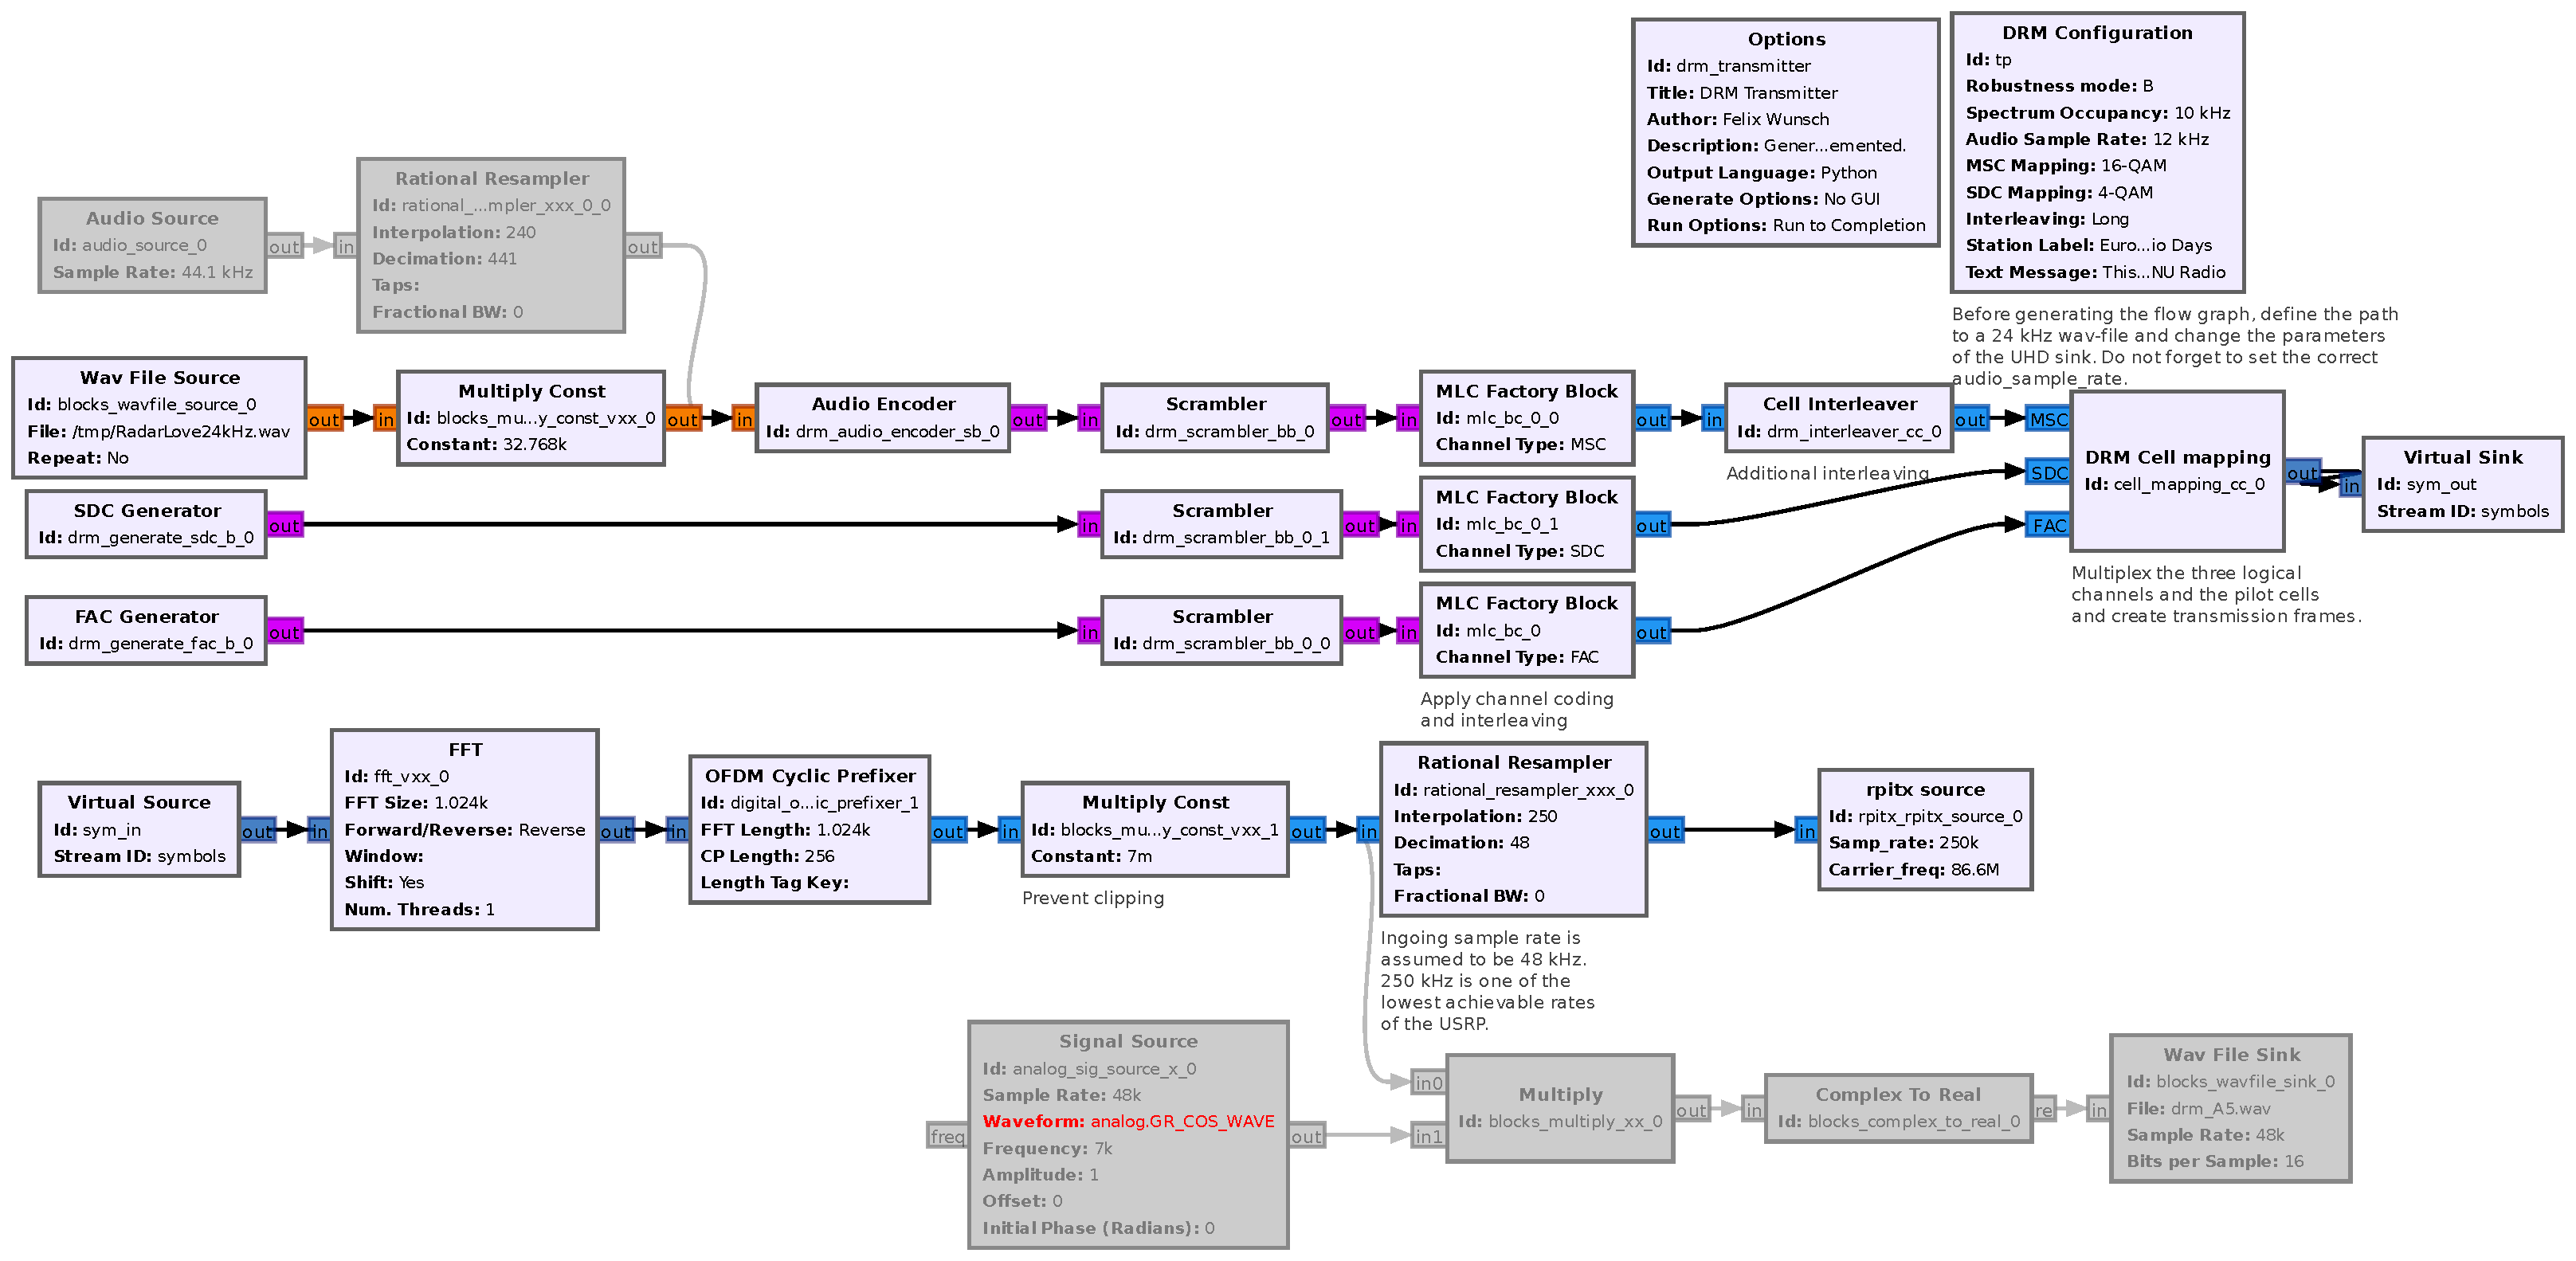
\includegraphics[width=\linewidth]{drm_transmitter.pdf}
\caption{Demonstration DRM flowchart as provided by {\tt gr-drm}, but replacing 
the USRP output with {\tt gr-rpitx}. Three datastreams -- FAC, SDC and MSC -- are 
summed and transmitted as the DRM signal, but only the first two will be demodulated
due to insufficient signal to noise ratio of the Raspberry Pi4 used as radiofrequency
transmitter.}
\label{drmtx}
\end{figure}

As demonstrated in Fig.
\ref{drm}, the simplest and sparsest modulation schemes are well decoded. Indeed, the Fast 
Acces Channel (encoded as 4-QAM, \url{https://www.drm-sender.de/?page=drm&lang=en#2_2}) 
and the Service Description Channel (SDR, also 4-QAM in this setting) exhibit good enough 
signal to noise ratio for analysis, while the Main Service Channel here encoded as 16-QAM 
and carrying the sound information cannot be decoded due to the insufficient signal to noise 
ratio to identify the symbols of this dense constellation.
Indeed with only 3-bit (7-levels) of amplitude tuning, {\tt gr-rpitx} lacks
the flexibility to address more advanced modulation schemes. This reception
scheme emphasizes how GNU Radio can benefit from external decoding software:
here DREAM (version 2.2.1 compiled using the instructions at
\url{https://gist.github.com/onetransistor/4cbe3a8ab5d47da22cde} since all
newer versions failed to run on a Debian/sid distribution as of this writing in
Summer 2021) expects a sound card input while GNU Radio streams a
sound card output. The link between the two is achieved with a virtual audio
cable created with Pulse Audio using
{\tt pactl load-module module-null-sink sink\_name=virtual 
sink\_properties=device.description="virtual"}. The Pulse Audio control softare
{\tt pavucontrol} then allows connecting the audio output of GNU Radio to this
virtual sink and feeding DREAM with this input stream.

\section{Dynamically tuning the carrier frequency: callback function}

GNU Radio users expect to be able to define the carrier frequency of
a sink block and dynamically tune this parameter e.g. through a slider
or by sending the new value through a client-server link. Dynamically
updating the parameter requires implementing a callback function: in this
case the {\tt set\_freq()} callback function will de-activate the DMA
stream, and re-activate the buffer with the new carrier frequency. Because
the sampling rate must be provided as argument, this value is saved as a 
private variable shared by all functions of the class
\begin{lstlisting}[language=C]
samp_rate_=samp_rate;
\end{lstlisting}
but furthermore, the work function must be prevented from writing in the DMA
buffer as reconfiguration is ongoing. A mutex (Mutually Exclusive) access is defined
to make sure that whenever the callback function is reconfiguring the DMA buffer,
the work function is prevented from writing as follows:
\begin{lstlisting}[language=C]
pthread_mutex_init(&th, NULL);
\end{lstlisting}
is defined in the constructor while the callback function defining the new carrier
frequency is
\begin{lstlisting}
void rpitx_source_impl::set_freq(float freq)
 {pthread_mutex_lock(&th);
  iqtest->stop();
  delete(iqtest);
  iqtest=new iqdmasync(freq,samp_rate_,\
         14,IQSize*4,MODE_IQ);
  iqtest->SetPLLMasterLoop(3,4,0);
  pthread_mutex_unlock(&th);
 }
\end{lstlisting}

with the main work function updated with
\begin{lstlisting}
while (nbread<noutput_items)
 {if (nbread+IQSize<noutput_items) 
     xferlen=IQSize; 
  else xferlen=noutput_items-nbread;
  pthread_mutex_lock(&th);
  iqtest->SetIQSamples((std::\
   complex<float>*)&in[nbread],xferlen,H);
  pthread_mutex_unlock(&th);
  nbread+=xferlen;
 }
\end{lstlisting}

This new structure is deleted in the destructor with
\begin{lstlisting}[language=C]
pthread_mutex_destroy(&th);
\end{lstlisting}

\section{Practical demonstration (3): scalar network analyzer}

As part of an undegraduate course on radiofrequency instrumentation,
we aimed at characterizing the transfer function of a dual-resonator
surface acoustic wave transducer designed to exhibit two resonances
around $434\pm 1$~MHz. Our initial investigation focused on a broadband
noise source as widely available by polarizing a Zener diode \cite{zener1,zener2},
but due to remote teaching conditions, the 12 to 24~V high voltage needed to 
power the noise generator was not available to most students assumed
to only have access to the 5~V output of a USB port. Hence, a noise source
generated by the Raspberry Pi(4) provided as recording platform was needed:
feeding a noise source IQ output to {\tt gr-rpitx} configured to operate
at 86.8~MHz would generate on its 5th overtone the required signal. Furthermore,
the documented 200~kHz sampling rate at fundamental mode (86.8~MHz) would extend
to 1~MHz on the 5th overtone, allowing to cover the whole Industrial, Scientific
and Medical (ISM) band with only two carried frequency shifts by 1~MHz/5=200~kHz.

Dynamic carrier frequency tuning is demonstrated at
\url{http://jmfriedt.free.fr/gr-rpitx_set_freq.mp4} and a sample measurement is
displayed in Fig. \ref{s21}.

\begin{figure}[h!tb]
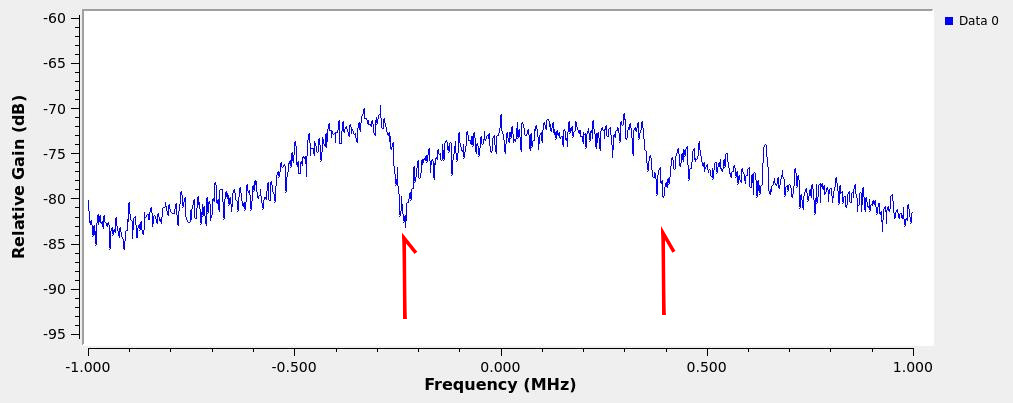
\includegraphics[width=\linewidth]{s21_SEAS10.jpg}
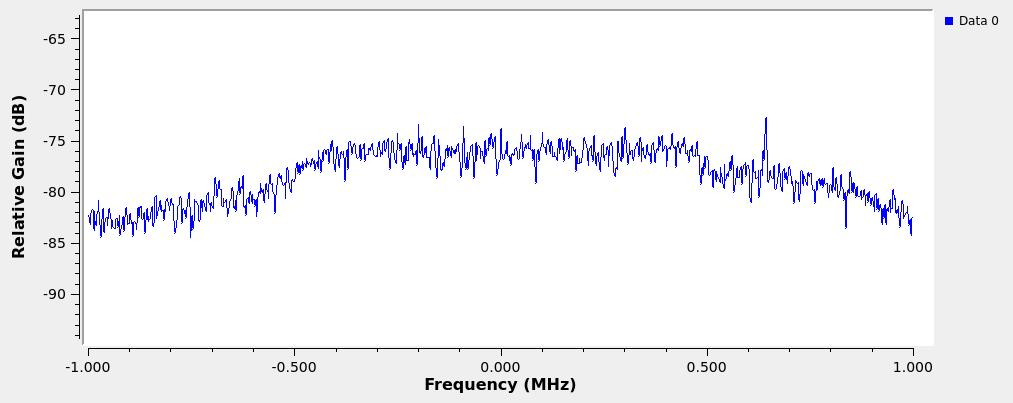
\includegraphics[width=\linewidth]{s21through.jpg}
\caption{Top: through configuration of the dual resonator SENSeOR (France) SEAS10 transducer
operating in the ISM band as cooperative target for passive, wireless sensing. Bottom: calibration
with a through measurement as reference when no sensor is present between the radiofrequency
output and the DVB-T receiver acting as general purpose software defined radio receiver. Arrows
on the top chart indicate the frequency offsets at which the resonance modes are observed.}
\label{s21}
\end{figure}

For comparison, the characterization of this same device using a Rohde \& Schwarz 
vector network analyzer is displayed in Fig. \ref{rs}.

\begin{figure}[h!tb]
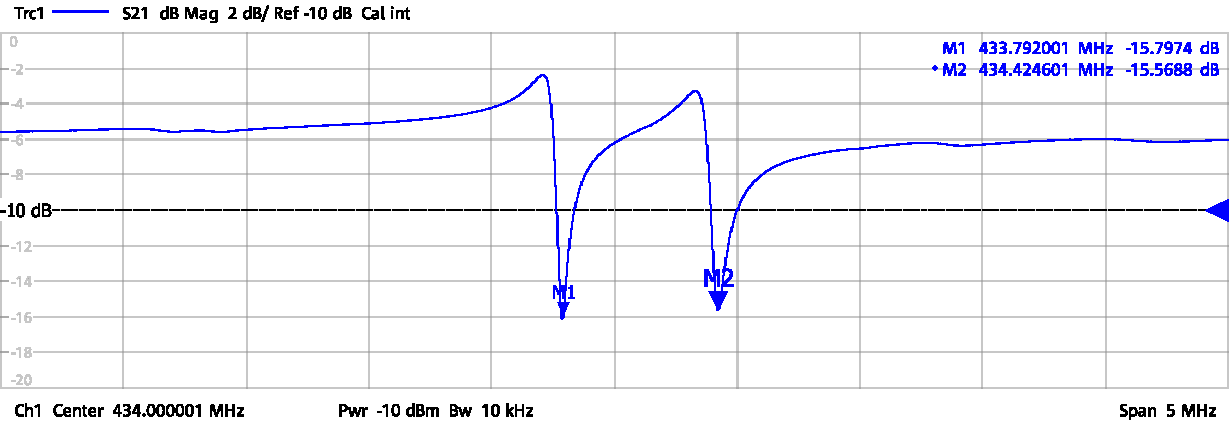
\includegraphics[width=\linewidth]{RetS.pdf}
\caption{Reference measurement of the SEAS10 transducer used in transmission mode in this 
experiment. The 5~MHz frequency span is broader than the chart displayed in Fig. \ref{s21}
to emphasize the lack of spurious resonance out of band.}
\label{rs}
\end{figure}

\section{Conclusion}

We have extended the capability of the Raspberry Pi(4) as a radiofrequency source
by providing compatibility with GNU Radio and hence all the signal processing
blocks available to generate signals as simple as broadcast analog frequency
modulated signals to as complex as Digital Radio Mondiale digital communication
streams. The emphasis is on educational purposes to promote investigations of
real signals plagued by practical issues such as fading and noisy communication
channels between the source and an inexpensive receiver such as a digital video
broadcast-terrestrial receiver used as general purpose software defined radio
receiver on the Raspberry Pi or the host personal computer.
The software is available at \url{https://github.com/jmfriedt/gr-rpitx}

\section*{Acknowledgement}

Emitting digital mode broadcast signal and using DRM for that purpose rather
than DAB(+) which would require excessive bandwidth was
supervised by Herv\'e Boeglen (XLim, Poitiers, France) who also improved the 
manuscript by proofreading.

\bibliography{gnuradiodays2021}
\bibliographystyle{grcon/grcon}

\end{document}

https://www.etsi.org/deliver/etsi_es/201900_201999/201980/03.01.01_50/es_201980v030101m.pdf

